\documentclass[14pt]{extarticle}
\usepackage{fontspec}
\usepackage{polyglossia} % use instead of babel
\usepackage{pgfplots}
\usepackage{float}
\usepackage{amsmath}
\usepackage{amsfonts}
\setdefaultlanguage{hebrew}
\setotherlanguage{english}
\newfontfamily\hebrewfont[Script=Hebrew]{Arial}

% TODO: figure out if better to keep this or not, for word document pdf output similarity
\usepackage[margin=1in]{geometry}

% might be useful to ensure similarity to word document pdf output
% \usepackage{setspace}
% \singlespacing

% Reset equation counter at the start of each section
\usepackage{chngcntr}
\usepackage{etoolbox}
\counterwithin*{equation}{section}
\preto{\section}{\setcounter{equation}{0}}

% Left-aligned equation environment
\newenvironment{lefteqs}{%
    \begin{english}%
    \begin{flushleft}%
    \renewcommand{\arraystretch}{1.3}%
    $\begin{array}{@{}l@{}}%
}{%
    \end{array}$%
    \end{flushleft}%
    \end{english}%
}

\begin{document}

\begin{center}
    {\LARGE \textbf{מעבדה 5}}\\
    {\textbf{גלי מיקרו}}
\end{center}

\begin{itemize}
    \item מגישים
    \begin{itemize}
        \item אורי כספי - 
        \item ארז - 
        \item שי רואימי - 318986270
    \end{itemize}
    \item תאריך ביצוע הניסוי: 27 ביולי 2026
\end{itemize}
\newpage
\section*{ניסוי 1 חלק 1 - חוק מאלוס}

\subsection*{מטרת הניסוי}
אימות חוק מאלוס עבור קיטוב קרינת מיקרו בעזרת משדר ומקלט המקוטבים קווית.

\subsection*{רקע תיאורטי}
גלי מיקרו הם גלים אלקטרומגנטיים באורך מספר סנטימטרים. אורך גל זה מאפשר בקלות יותר לחקור את התנהגות הגלים.

גל אלקטרומגנטי מישורי מתואר על ידי וקטור השדה החשמלי $\vec{E}$ המתנודד בכיוון קבוע במישור הניצב לכיוון ההתקדמות.  
כיוון הקיטוב של הגל מוגדר בתור כיוון השדה החשמלי.
גל בו כיוון הקיטוב קבוע נקרא גל מקוטב קווית.

מקלט מקוטב קולט רק את היטל השדה החשמלי על ציר הקליטה שלו. אם השדה הפוגע הוא $\vec{E}$ בעל משרעת $E_0$, וזווית הקיטוב שלו סוטה בזווית $\theta$ מציר הקליטה,
אז משרעת הרכיב הנקלט היא:
\begin{equation}
    E = E_0 \cos(\theta)
\end{equation}
כאשר $E_0$ משרעת השדה היוצא מהמשדר, ו $\theta$ הזווית בין כיוון הקיטוב של המשדר לציר הקליטה של המקלט.

עוצמת הגל מתכונתית לריבוע השדה החשמלי: $I \propto E^2$, וכן חוק מאלוס קובע:
\begin{equation}
    I = I_0 \cos^2(\theta)
\end{equation}
כאשר $I$ העוצמה הנקלטת, ו $I_0$ היא העוצמה הנקלטת כאשר כיווני המשדר והמקלט מקבילים ($\theta = 0$).

\subsection*{מערכת המדידה ומהלך הניסוי}

הרכבנו משדר ומקלט (המשדר פולט גלי מיקרו מקוטבים קווית בתדר $10.525GHz$) על מסילה (מקובעים).

שני המכשירים (מקלט ומשדר) היו ניתנים לסיבוב סביב הציר האופטי כאשר היה מד זווית בגב כל מכשיר ככה שניתן היה לקרוא את זווית הקיטוב.

למקלט יש מד זרם אנלוגי המציג את מדידת עוצמת הגל הנקלט.

בחלק השני של הניסוי נוסף למערכת סריג מתכתי שהצבנו בין על המסילה בין המשדר למקלט.

יש לציין שעל מנת למנוע הפרעות במדידות השתדלנו להסיר חפצים מתכתיים מהסביבה.

אתחלנו את שני מדי הזווית (של המשדר והמקלט) לזווית אפס, כך שכיוון הקיטוב של המשדר והמקלט מקבילים.

השארנו את המקלט קבוע בזווית אפס, ואת המשדר סובבנו בקפיצות של $10^\circ$ עד שהגענו לזווית $90^\circ$.

בכל זווית רשמנו את קריאת מד הזרם.

\subsection*{תוצאות וניתוח}

תוצאות המדידה של הזרם במקלט כפונקציה של זווית הקיטוב של המשדר מוצגות בטבלה:

\begin{table}[H]
    \centering
    \renewcommand{\arraystretch}{1.5} % Increase row height
    \begin{tabular}{|c|c|c|c|}
        \hline
        \text{$\cos^2(\theta)$} & \text{$\frac{I}{I_{max}}$} &\text{[mA] $I$}& \text{[מעלות] $\theta$} \\ \hline
        1 & 1 & 156 & $0^\circ$ \\ \hline
        0.969 & 0.961 & 150 & $10^\circ$ \\ \hline
        0.883 & 0.923 & 144 & $20^\circ$ \\ \hline
        0.75 & 0.884 & 138 & $30^\circ$ \\ \hline
        0.587 & 0.807 & 126 & $40^\circ$ \\ \hline
        0.413 & 0.692 & 108 & $50^\circ$ \\ \hline
        0.25 & 0.538 & 84 & $60^\circ$ \\ \hline
        0.117 & 0.365 & 57 & $70^\circ$ \\ \hline
        0.03 & 0.192 & 30 & $80^\circ$ \\ \hline
        0 & 0 & 0 & $90^\circ$ \\ \hline
    \end{tabular}
    \caption{מדידת זרם במקלט כפונקציה של זווית הקיטוב של המשדר}
    \label{tab:malus_p1}
\end{table}

\begin{figure}[H]
    \centering
    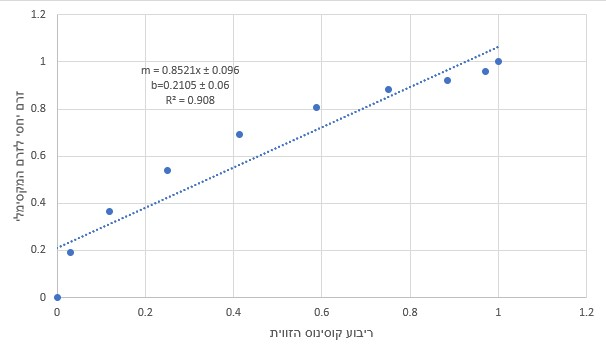
\includegraphics[width=0.8\textwidth]{E1_part_1.jpg}
    \caption{גרף של $\frac{I}{I_{max}}$ כפונקציה של $\cos^2(\theta)$}
\end{figure}

מדדנו את זרם המקלט $I$ כפונקציה של הזווית $\theta$ בקפיצות של $10^\circ$

את הזרם היחסי חישבנו ביחס לזרם המירבי $I_{max} = 156 mA$ שהתקבל עבור $\theta = 0^\circ$.

לפי חוק מאלוס, צפינו לקבל קו ישר בעל שיפוע 1 וחיתוך ציר $y$ ב $y=0$.

מהתאמת קו מגמה למדידות קיבלנו שיפוע $m=0.852, b=0.2105$.

חישבנו את שגיאת השיפוע לפי נוסחת הרגרסיה הלינירית (נוסחא 17 בתדריך השגיאות):

\begin{lefteqs}
    \Delta y = \sqrt{\frac{1}{N-2} \sum (y_i - m x_i - b)^2} \\
    \Delta m = \Delta y \sqrt{\frac{N}{A}} \\
    \Delta b = \Delta y \sqrt{\frac{S_{xx}}{A}} \\
    A = N S_{xx} - S_x^2 \\
    S_{xx} = \sum x_i^2 \\
    S_x = \sum x_i \\
\end{lefteqs}

כאשר $\Delta y$ מאפיין את סטיית הנקודות מקו המגמה, $N=10$ כמספר המדידות, ו $A$ מבטא את פיזור ערכי $x$.

הערכים חושבו באמצעות פונקציית LINEST באקסל המיישמת נוסחא זו:
\begin{lefteqs}
    \Delta y = 0.112 \\
    \Delta m = 0.096 \\
    \Delta b = 0.06
\end{lefteqs}

כלומר (בעיגול בהתאם לגודל השגיאה):

\begin{lefteqs}
    m = 0.85 \pm 0.10 \\
    b = 0.21 \pm 0.06
\end{lefteqs}

יש לציין כי נוסחא (17) מניחה $\Delta x << \Delta y$, ובמקרה שלנו $\Delta x$ (הנובע משגיאת הזווית של $\cos^2(\theta)$) אינו זניח לחלוטין סביב $\theta = 45^\circ$ אך אינו משנה את המסקנות.

שגיאות המדידה במד הזרם ומד הזווית נכללות במילא בפיזור הנקודות סביב קו המגמה ולכן שגיאת הרגרסיה מייצגת את אי-הוודאות הסטטיסטית הכוללת בשיפוע.

השגיאה היחסית של השיפוע היא:
\begin{lefteqs}
    \frac{\Delta m}{m} = \frac{0.096}{0.852} = 0.11 \approx 11\%
\end{lefteqs}

שגיאת יחסית זו קטנה מהסף המקובל ($20-25\%$) ולכן תוצאת המדידה משמעותית.

הערך הצפוי לפי חוק מאלוס הוא 1, הסטייה בין התוצאה לערך הצפוי היא:
\begin{lefteqs}
    \frac{|m - 1|}{1} = |0.852 - 1| \approx 0.15
\end{lefteqs}

כלומר סטייה יחסית של $15\%$ ביחס לערך הצפוי.

הערך הצפוי 1 נופל מעט מחוץ לטווח $m \pm \Delta m = [0.75, 0.95]$ - הסטייה גדולה מהשגיאה המוערכת.

גם החיתוך שהתקבל $b=0.21 \pm 0.06$ חורג מהערך הצפוי 0.

מקור הסטייה מצוין בתדריך הניסוי: מד הזרם במקלט אינו מתכונתי במדויק לעוצמת הגל ($E^2$),
אלא נמצא בתחום ביניים בין תלות בעוצמה לתלות בשדה ($E$).
הסטייה שהתקבלה עקבית עם אי־התאמה זו: גלאי מתכונתי לעוצמה היה נותן קו ישר בעל שיפוע  1
ואילו תגובה הנוטה לכיוון תלות בשדה היא קעורה כנגד $\cos^2(\theta)$ - 
וזו בדיוק צורת השאריות שנצפתה, הכופה שיפוע קטן מ-1 וחיתוך גדול מ-0.

\subsection*{דיון ומסקנות}
התוצאה הסופית שהתקבלה היא:
\begin{lefteqs}
    m = 0.85 \pm 0.10 \\
    b = 0.21 \pm 0.06
\end{lefteqs}

ע"פ חוק מאלוס צפינו לקבל שיפוע 1 וחיתוך 0, כאשר הערך 1 נופל מחוץ לטווח השגיאה [0.75, 0.95], בסטייה של $15\%$.

הגרף ליניארי בקירוב אך לא לגמרי, השאריות מסודרות בדפוס קעור. הנקודות מעל קו ההתאמה במרכז התחום ומתחתיו בקצוות.
כלומר הסטייה היא שיטתית ולא אקראית.

לכן העובדה שהערך הצפוי נופל מחוץ לטווח השגיאה אינה מעידה על הפרת חוק מאלוס אלא על כך שמודל קו ישר אינו מתאים לצורת הנתונים.
הסיבה הפיזיקלית לעקומומיות (תגובת מד זרם שאינה מתכונתית לעוצמה) מפורטת בניתוח התוצאות.

\newpage


\section*{ניסוי 1 חלק 2 - קיטוב ע"י סריג מתכתי}
\subsection*{מטרת הניסוי}
חקירת תכונות סריג מתכתי בתור מקטב עבור קיטוב קרינת מיקרו בעזרת משדר ומקלט המקוטבים קווית.

\subsection*{רקע תיאורטי}
בנוסף לרקע התיאורטי עבור חלק 1 של הניסוי,  הסריג המשמש כמקטב בניסוי הוא מערך של תילים מוליכים מקבילים, שהמרחק ביניהם קטן מאורך הגל.
פעולתו נובעת מהיענות האלקטרונים בתילים לשדה הפוגע:

\begin{itemize}
    \item 
כאשר כיוון הקיטוב מקביל לתילים, האלקטרונים מואצים חופשית לאורך התיל ומשדרים מחדש קרינה מפוזרת. הקרינה המפוזרת מתאבכת באופן הורס עם הקרינה הפוגעת בכיוון ההתקדמות, והרכיב הזה נחסם (מוחזר לאחור).
    \item
כאשר כיוון הקיטוב ניצב לתילים, תנועת האלקטרונים מוגבלת (עובי התיל קטן מאורך הגל), כמעט אין קרינה מפוזרת, והרכיב הזה עובר כמעט ללא הפרעה.
\end{itemize}

נגדיר את $\theta$ בתור הזווית בין כיוון הקיטוב (משותף למשדר ולמקלט) לבין כיוון התילים.
כאשר $\theta = 0$ הקיטוב מקביל לתילים והקרינה נחסמת.

כאשר פוגע בסריג שדה בעל משרעת $E_0$, בזווית $\theta$, הסריג מעביר רק את הרכיב הניצב, בעל משרעת:
\begin{equation}
    E_1 = E_0 \sin(\theta)
\end{equation}

מכיוון שציר הקליטה של המקלט נמצא בזווית $\theta$ מכיוון התילים, הזווית בינו לבין השדה היוצא (ניצב לתילים) היא $\theta - 90^\circ$, ולכן המשרעת הנקלטת היא:
\begin{equation}
    E_2 = E_1 \cos(90^\circ - \theta) = E_0 \sin(\theta) \sin(\theta) = E_0 \sin^2(\theta)
\end{equation}

מכיוון ש $I \propto E^2$, נקבל את עוצמת האור הנקלט:
\begin{equation}
    I = I_0 \sin^4(\theta) \Rightarrow \frac{I}{I_{max}} = \sin^4(\theta)
\end{equation}

כאשר $I_{max}$ היא העוצמה הנקלטת המרבית כאשר $\theta = 90^\circ$.

\subsection*{מערכת המדידה ומהלך הניסוי}

מערכת המדידה זהה לזהו שתוארה בחלק 1 של הניסוי, בתוספת סריג מתכתי (מערך תילים מוליכים מקבילים)
שהוצב על המסילה בין המשדר למקלט.

הצבנו את הסריג המתכתי בין המשדר למקלט כך שבמצב ההתחלתי התילים מקבילים לכיוון הקיטוב המשותף של המשדר והמקלט.

במצב זה הזרם הנמדד היה אפס.

לאחר מכן סובבנו את המשדר והמקלט יחד בקפיצות של $10^\circ$ עד שהגענו לזווית $90^\circ$.

גם כאן, נרשם הזרם הנמדד בכל זווית.

\subsection*{תוצאות וניתוח}

תוצאות המדידה של הזרם במקלט כפונקציה של זווית המשדר והמקלט ביחס לכיוון התילים מוצגות בטבלה:

\begin{table}[H]
    \centering
    \renewcommand{\arraystretch}{1.5} % Increase row height
    \begin{tabular}{|c|c|c|c|}
        \hline
        \text{$\sin^4(\theta)$} & \text{$\frac{I}{I_{max}}$} &\text{[mA] $I$}& \text{[מעלות] $\theta$} \\ \hline
        0 & 0.004 & 0.06 & $0^\circ$ \\ \hline
        0.001 & 0.004 & 0.06 & $10^\circ$ \\ \hline
        0.0137 & 0.039 & 0.54 & $20^\circ$ \\ \hline
        0.0625 & 0.145 & 2.01 & $30^\circ$ \\ \hline
        0.1707 & 0.289 & 4 & $40^\circ$ \\ \hline
        0.344 & 0.449 & 6.2 & $50^\circ$ \\ \hline
        0.5625 & 0.594 & 8.2 & $60^\circ$ \\ \hline
        0.78 & 0.826 & 11.4 & $70^\circ$ \\ \hline
        0.94 & 0.935 & 12.9 & $80^\circ$ \\ \hline
        1 & 1 & 13.8 & $90^\circ$ \\ \hline
    \end{tabular}
    \caption{מדידת זרם במקלט כפונקציה של זווית הקיטוב של המשדר}
    \label{tab:malus_p1}
\end{table}

\begin{figure}[H]
    \centering
    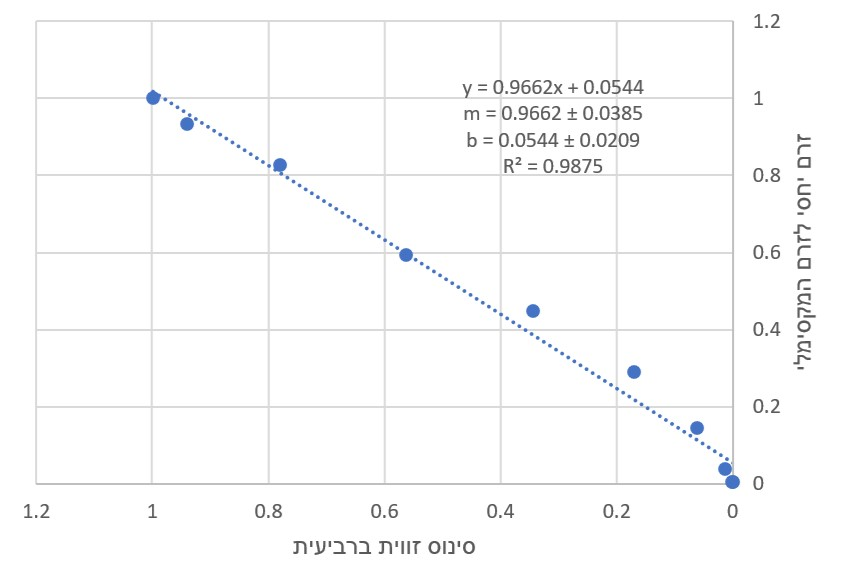
\includegraphics[width=0.8\textwidth]{E1_part_2.jpg}
    \caption{גרף של $\frac{I}{I_{max}}$ כפונקציה של $\sin^4(\theta)$}
\end{figure}

גם בחלק זה מדדרנו את הזרם במקלט כפונקציה של הזווית $\theta$ בקפיצות של $10^\circ$.
את הזרם היחסי חישבנו ביחס לזרם המיקרבי $I_{max} = 13.8 mA$ שהתקבל עבור $\theta = 90^\circ$.

התאמת קו מגמה נותן לנו את השיפוע $m=0.9662$, וחיתוך עם ציר $y$ ב $b=0.0544$.

את השגיאה נחישבנו באותו אופן כמו בחלק 1 של הניסוי (נוסחא 17 מפרק השגיאות, כאשר הערכים חושבו ע"י פונקציית LINEST ב Excel המיישמת  נוסחא זו), וקיבלנו:
\begin{lefteqs}
    \Delta y = 0.046 \\
    \Delta m = 0.038 \\
    \Delta b = 0.021
\end{lefteqs}

\subsection*{דיון ומסקנות}
בנקודה (1) במהלך הניסוי נשאלנו מה עוצמת הגל הנקלט כאשר רצועות הסריג מקבילות לכיוון הקיטוב של המשדר, ומדוע.

כפי שהוסבר ברקע התיאורטי, כאשר כיוון הקיטוב מקביל לתילים, האלקטרונים מואצים חופשית לאורך התיל ומשדרים מחדש קרינה מפוזרת. הקרינה המפוזרת מתאבכת באופן הורס עם הקרינה הפוגעת בכיוון ההתקדמות, והרכיב הזה נחסם (מוחזר לאחור). לכן העוצמה הנקלטת היא אפס.

התוצאה הסופית שהתקבלה היא:
\begin{lefteqs}
    m = 0.966 \pm 0.038 \\
    b = 0.054 \pm 0.021
\end{lefteqs}

הגרף שקיבלנו ליניארי במידה טובה: מקדם המתאם הוא $R^2 = 0.975$, והשיפוע מכיל בטווח השגיאה שלו
את הערך הצפוי 1 (טווח השגיאה הוא [0.928, 1.004]).

השגיאה היחסית של השיפוע היא:
\begin{lefteqs}
    \frac{\Delta m}{m} = \frac{0.038}{0.966} = 0.039 \approx 4\%
\end{lefteqs}

הסטייה מהערך הצפוי היא:
\begin{lefteqs}
    \frac{|m - 1|}{1} = |0.966 - 1| \approx 0.034
\end{lefteqs}

כלומר סטייה יחסית של $3.4\%$ ביחס לערך הצפוי, כלומר השגיאה קטנה מהסטייה, ולכן התוצאה משמעותית.

החיתוך שהתקבל $b=0.054 \pm 0.021$ חורג מעט מהערך הצפוי (הערך 0 נופל מחוץ לטווח השגיאה).
סטייה זו עקבית עם אותו מקור שיטתי שזוהה בחלק 1: מד הזרם אינו מתכונתי במדויק לעוצמה ותגובתו הלא-ריבועית גורמת לעקמויות קלה בנתנונים הדוחפת את החיתוך מעט מעל 0.

לסיכום, התוצאות מאשרות את הנוסחא.

\newpage
\section*{ניסוי 2 - התאבכות משני סדקים}

\subsection*{מטרת הניסוי}
1. לצפות בהתאבכות של גלי מיקרו דרך שני סדקים
2. מדידת אורך גל של קרינת מיקרו בעזרת בחינת תבנית ההתאבכות

\subsection*{רקע תיאורטי}
בניסוי זה אנחנו עובדים עם גלי מיקרו בעלי אורך גל מסדר גודל של סנטימטרים.

עובדה וז מאפשרת לראות תופעות התאבכות קלאסיות בסקאלה מאקרוסקופית.
על מנת שהתופעה תהיה נצפית צריך שהממדים הגיאומטריים של המערכת יהיו בסדר גודל של אורך הגל (מספר סנטימטרים).

כאשר שני גלים אלקטרומגנטיים בעלי אותו תדר מגיעים לאותה נקודה, שדותיהם מתחברים לפי עקרון הסופרפוזיציה.
העוצמה בנקודה נקבעת ע"פ הפרש המופע בין הגלים, שנקבע על ידי הפרש הדרכים שעברו.

על מנת שתבנית ההתאבכות תהיה יצירה בזמן, שני המקורות צריכים להיות קוהרנטיים (בעלי הפרש מופע קבוע).
בניסוי זה שני הסדקים מוארים על ידי אותו גל מישורי הנפלט מאותו מקור, ולכן הם קוהרנטיים.

לפי עקרון הויגנס כל סדק משמש מקור משני ושני המקורות המשניים חולקים את אותה פאזה.

תהי $\theta$ הזווית ביחס לציר האופטי (נומרל למישור הסדקים).
במרחק גדול מספיק מן הסדקים (הקירוב הפאראקסיאלי), התאבכות בונה מתקבלת כאשר הפרש הדרך שווה לכפולה שלמה של אורך הגל:

\begin{equation}
    d \sin(\theta_n) = n \lambda \, ,n=0,\pm 1, \pm 2, \ldots
\end{equation}

והתאבכות הורסת מתקבלת כאשר הוא שווה לכפולה אי זוגית של חצי אורך גל:
\begin{equation}
    d \sin(\theta_n) = (n + \frac{1}{2}) \lambda
\end{equation}

כאשר $\lambda$ אורך הגל, $d$ המרחק בין מרכזי הסדקים, ו $\theta_n$ הזווית שבה מופיע המקסימום מסדר $n$ ביחס לציר האופטי, ו-$n$ סדר המקסימום.

את אורך הגל ניתן לחלץ מזווית מקסימום שנמדדה:

\begin{equation}
    \lambda = \frac{d \sin(\theta_n)}{n}
\end{equation}

\subsection*{מערכת המדידה ומהלך הניסוי}

המשדר והמקלט נמצאו על אותו סרגל אופטי לאחר ניסוי 1. ביניהם הרכבנו על הסרגל לוח עליו מודפסים שני סדקים רחבים.
מדדנו את המרחק בין הסדקים, והוא $5.9cm \pm 0.1cm$.

כיוונו את המשדר והמקלט כך שכיווני הקיטוב שלהם יהיו מאונכים לסדקים. הסבר מדוע מופיע בדיון ומסקנות.

לאחר מכן סובבנו את הציר שעליו יושב המקלט (שינוי הזווית $\theta$) עד שמצאנו משני הצדדים של הציר את זוויות המקסימום הראשונות (סדר 1) של הקרינה הנקלטת.

\subsection*{תוצאות וניתוח}

מדידות הזרם במקלט עבור הזוויות בהן מדדנו:

\begin{table}[H]
    \centering
    \renewcommand{\arraystretch}{1.5} % Increase row height
    \begin{tabular}{|c|c|}
        \hline
        \text{[מעלות] $\theta$} & \text{[mA] $I$} \\ \hline
        $0^\circ$ & 7.6 \\ \hline
        $22^\circ$ & 7.2 \\ \hline
        $-23^\circ$ & 7.2 \\ \hline
    \end{tabular}
    \caption{מדידת זרם במקלט עבור זוויות שונות}
    \label{tab:l5_e2}
\end{table}

נשים לב כי שני המסקימומים מסדר ראשון נמדדו בעוצמה זהה, שקטנה מהעוצמה במרכז.

את אורך הגל נחשב בעזרת נוסחא (3) לשתי הזוויות בהן נמדד מקסימום מסדר 1:

\begin{lefteqs}
    \lambda_{n=1} = \frac{d \sin(\theta_1)}{1} = 5.9cm \cdot \sin(22^\circ) = 2.21cm \\
    \lambda_{n=-1} = \frac{d \sin(\theta_{-1})}{-1} = -1 \cdot 5.9cm \cdot \sin(-23^\circ) \approx 2.30cm
\end{lefteqs}

הערך הטוב ביותר לאורך הגל הוא ממוצע שתי המדידות:
\begin{lefteqs}
    \bar{\lambda} = \frac{\lambda_{n=1} + \lambda_{n=-1}}{2} = 2.255cm \approx 2.26cm
\end{lefteqs}

ע"פ נוסחא (2) בפרק השגיאות, השגיאה הסטטיסטית בניסוי בו נעשו מספר מדידות היא:
\begin{lefteqs}
    \Delta \lambda = \sqrt{\frac{\Sigma_i^N (\lambda_i - \bar{\lambda})^2}{N}}
\end{lefteqs}

כלומר השגיאה הסטטיסטית היא:
\begin{lefteqs}
    \Delta \lambda = \sqrt{\frac{(2.21 - 2.255)^2 + (2.3 - 2.255)^2}{2}} = 0.045cm \approx 0.05cm
\end{lefteqs}

ולכן התוצאה הסופית היא:
\begin{lefteqs}
    \lambda = 2.26 \pm 0.05cm
\end{lefteqs}

\subsection*{דיון ומסקנות}

מדידת אורך הגל של קרינת המיקרו נתנה:
\begin{lefteqs}
    \lambda = 2.26 \pm 0.05cm
\end{lefteqs}

המשדר פועל בתדר קבוע ידוע $f=10.525Gh$ ולכן אורך הגל הצפוי בריק הוא:

\begin{lefteqs}
    \lambda_{expected} = \frac{c}{f} = \frac{3 \cdot 10^8 m/s}{10.525 \cdot 10^9 Hz} = 2.85cm
\end{lefteqs}

הסטייה היחסית של התוצאה הנמדדת מאורך גל זה היא:

\begin{lefteqs}
    \frac{|\lambda_{expected} - \lambda|}{\lambda_{expected}} = \frac{|2.85 - 2.26|}{2.85} \approx 21 \%
\end{lefteqs}

הערך התיאורטי $2.85cm$ נמצא מחוץ לטווח השגיאה $[2.21, 2.31]cm$ ולכן המדידה אינה מסכימה עם הערך הצפוי.

לפי נוסחא (3), על מנת לקבל את אורך הגל התיאורטי עם $d=5.9cm$, המקסימום הראשון היה צריך להופיע בזווית:
\begin{lefteqs}
    \theta_{expected} = \arcsin(\frac{\lambda_{exppected}}{d}) = \arcsin(\frac{2.85}{5.9}) \approx 29^\circ
\end{lefteqs}
ואילו אצלינו נמדדה זווית של $22^\circ$ ו $23^\circ$.
כלומר הזוויות שנמדדו קטנות באופן שיטטי בכ $6-7^\circ$ מהזווית הצפויה.

הסיבה העיקרית היא שבגלי מיקרו המקסימומים הם רחבים. אורך הגל הוא מסדר גודל של ממדי המערכת,
ולכן הפיזור הזויתי גדול ושיר והשיא מרוח על פני תחום זוויות שקשה לאתר את מרכזו במדויק.

סיבה אפשרית נוספת היא החזרת גלים מעצמים באזור הניסוי, שהשפיעו על עוצמת הגל הנמדדת ע"י התאבכות.

בתחילת הניסוי כיוונו את המשדר והמקלט כך שכיווני הקיטוב שלהם מאונכים לסדקים.
לוח הסדקים היה עשוי מתכת, והמתכת שסביב כל סדק מעבירה או חוסמת את הגל בהתאם לכיוון הקיטוב.
כאשר השדה החשמלי מקביל לסדקים, הוא מניע את האלקטרונים לאורך שפות המתכת של הסדק,
 ואז האלקטרונים המואצים משדרים קרינה מפורזת שמתאבכת באופן הורס עם הקרינה הפוגעת והלוח חוסם את הגל.

 לעומת זאת, כאשר השדה החשמלי מאונך לסדקים, תנועת האלקטרונים לרוחב מוגבלת כך שכמעט ואין קרינה מפוזרת והגל עובר בין הסדקים.

 כלומר כאשר הקיטוב מאונך לסדקים הקרינה תקלט במקלט בעוצמה מרבית.

נוסף על כך, יש לציין כי שני המקסימומים מסדר ראשון נמדדו בעוצמה זהה (7.2mA) שקטנה מהמרכז (7.6mA), כמצופה.
הסיבה היא שתבנית ההתאבכות של שני הסדקים יושבת מתחת למעטפת עקיפה של סדק יחיד שנקבעת ע"פ רוחב הסדק הבודד.
מעטפת זו דועכת ככל שמתרחקים מהציר האופטי ולכן מקסימומי ההתאבכות הרחוקים מהמרכז חלשים יותר.
כלומר, $d$ קובע היכן נמצאים השיאים, ו $a$ (רוחק הסדק) קובע את עוצמתם היחסית דרך המעטפת.

\end{document}


\end{document}
